\documentclass[12pt]{article}
\usepackage[russian]{babel}
\usepackage{geometry}

\usepackage{graphicx} % вставка изображений
\usepackage{caption} % описание изображений

%различные цветовые модели
\usepackage[usenames]{color}
\usepackage[dvipsnames,table]{xcolor}
\usepackage{colortbl}

\usepackage{tikz}
\usetikzlibrary{shapes, arrows}
\usepackage{varwidth}
\usepackage{ifthen}

\usepackage{enumitem}

\usepackage{multicol} % вставка изображений в две колонки
\usepackage{makecell} % вставка изображений в две колонки


%циклы foreach в tikz и создание переменных внутри этого окружения
\usepackage{pgffor}
\usepackage{pgfmath}

\usepackage{xifthen}

\usepackage{afterpage}

\usepackage{amssymb}
\usepackage{amsmath}

\usepackage{hyperref}

\usepackage[utf8]{inputenc}

\tikzstyle{connector} = [draw, -latex']
\tikzstyle{line} = [draw, -]
\tikzstyle{dashed} = [draw, -, dash pattern=on 5pt off 5pt]


\usepackage{listings}
\usepackage{listingsutf8}
\usepackage[T2A]{fontenc}
\newcommand{\listingsttfamily}{\usefont{T2A}{PTMono-TLF}{m}{n}}

\lstset{
	language=C,                % choose the language of the code
	numbers=left,                   % where to put the line-numbers
	stepnumber=1,                   % the step between two line-numbers.        
	numbersep=5pt,                  % how far the line-numbers are from the code
	backgroundcolor=\color{black},  % choose the background color. You must add \usepackage{color}
	commentstyle=\color{Gray},
	basicstyle=\listingsttfamily\color{Gray},
	keywordstyle=\color{BurntOrange},
	stringstyle=\color{YellowGreen},
	showspaces=false,               % show spaces adding particular underscores
	showstringspaces=false,         % underline spaces within strings
	showtabs=false,                 % show tabs within strings adding particular underscores
	tabsize=4,                      % sets default tabsize to 2 spaces
	captionpos=b,                   % sets the caption-position to bottom
	breaklines=true,                % sets automatic line breaking
	breakatwhitespace=true,         % sets if automatic breaks should only happen at whitespace
	title=\lstname, 
	inputencoding=utf8,                % show the filename of files included with \lstinputlisting;
	extendedchars=\true,
	keepspaces=true
}

\geometry{top=2cm, bottom=2cm, left=3cm, right=1.5cm}
\textheight=24cm
\textwidth=18cm
\flushbottom 

\oddsidemargin=0pt 
\topmargin=-1.5cm 
\parskip=0.25cm
\parindent=24pt 

\tolerance=2000 

\setcounter{secnumdepth}{0}

\setlist[1]{noitemsep} % sets the itemsep and parsep for all level two lists to 0

\begin{document}
	\begin{center}
		{\parskip=1cm
			МИНИСТЕРСТВО НАУКИ И ВЫСШЕГО ОБРАЗОВАНИЯ РОССИЙСКОЙ ФЕДЕРАЦИИ
			
			ФЕДЕРАЛЬНОЕ ГОСУДАРСТВЕННОЕ БЮДЖЕТНОЕ ОБРАЗОВАТЕЛЬНОЕ УЧРЕЖДЕНИЕ ВЫСШЕГО ОБРАЗОВАНИЯ
			
			{\bf«БЕЛГОРОДСКИЙ ГОСУДАРСТВЕННЫЙ ТЕХНОЛОГИЧЕСКИЙ УНИВЕРСИТЕТ им. В. Г. Шухова»\\(БГТУ им. В. Г. Шухова)}
			
			\begin{figure}[bh]
				\noindent\centering{
					
\includegraphics[width=100mm]{images/start_logo.png}
					\captionsetup{labelformat=empty}
				}
			\end{figure}
			Кафедра программного обеспечения вычислительной техники и автоматизированных систем
		}
		
		{\Large 
			\vspace{1cm}
			{\parskip=0.25cm 
				{\bf Лабораторная работа №4.1}
				
				по дисциплине: «Дискретная математика»
				
				по теме: {\bf Графы, маршруты}
			}
		}
	\end{center}	
	\begin{flushleft}
		{\leftskip=10cm
			{\vspace{3cm} Выполнил/a: ст. группы ПВ-231}
			
			Чупахина София Александровна
			
			Проверил: Рязанов Юрий Дмитриевич
			
		}
	\end{flushleft}
	\begin{center}
		{\parskip=3cm Белгород, 2024}
	\end{center}
	\newpage

	\tableofcontents
	
	\vspace{1cm}
	
	{\Large \bf Вариант 6}
	 
	\begin{description}
	\item [а)] Матрица смежности графа $G_1$:
	
	 $$
	 \left(\begin{tabular}{c c c c c c c}
	 	0 & 1 & 0 & 1 & 0 & 1 & 1 \\
	 	1 & 0 & 1 & 1 & 0 & 0 & 0 \\
	 	0 & 1 & 0 & 1 & 1 & 1 & 0 \\
	 	1 & 1 & 1 & 0 & 0 & 0 & 0 \\
	 	0 & 0 & 1 & 0 & 0 & 1 & 0 \\
	 	1 & 0 & 1 & 0 & 1 & 0 & 1 \\
	 	1 & 0 & 0 & 0 & 0 & 1 & 0 \\
	 	\end{tabular}
	 \right)
	$$
	Диаграмма графа $G_2$: 
	
	\begin{figure}[!h]
	\centering
	\begin{tikzpicture}{line width=3pt}
	\def\step{2}
	\node[circle, draw=black, minimum height=1cm] at (-2*\step, 0) (knot1) {1};
	\node[circle, draw=black, minimum height=1cm] at (0, 0) (knot6) {6};
	\node[circle, draw=black, minimum height=1cm] at (2*\step, 0) (knot4) {4};
	
	\node[circle, draw=black, minimum height=1cm] at (-\step, \step) (knot2) {2};
	\node[circle, draw=black, minimum height=1cm] at (\step, \step) (knot3) {3};

	\node[circle, draw=black, minimum height=1cm] at (-\step, -\step) (knot7) {7};
	\node[circle, draw=black, minimum height=1cm] at (\step, -\step) (knot5) {5};
	
	\path[line, line width = 1.25pt] (knot1) -- (knot2);
	\path[line, line width = 1.25pt] (knot1) -- (knot7);		
	\path[line, line width = 1.25pt] (knot2) -- (knot6);							
	\path[line, line width = 1.25pt] (knot7) -- (knot6);
	
	\path[line, line width = 1.25pt] (knot6) -- (knot3);
	\path[line, line width = 1.25pt] (knot6) -- (knot5);		
	\path[line, line width = 1.25pt] (knot3) -- (knot4);							
	\path[line, line width = 1.25pt] (knot5) -- (knot4);
	\end{tikzpicture}
	\end{figure}

	\item[б)] Последовательности вершин:
	\begin{enumerate}
	\item(1, 7, 6, 3, 5)
	\item(6, 5, 3, 6, 7, 1) 
	\item(7, 6, 3, 2, 1, 7) 
	\item(4, 3, 5, 3, 6, 5) 
	\item(1, 2, 7, 6, 2, 1) 
	\end{enumerate}
	
	\end{description}

	\section{Задание 1}
	\label{task1}
	{\bf Текст задания:} Представить графы $G_1$ и $G_2$ (см. <<Варианты заданий>>, п.а) матрицей смежности, матрицей инцидентности, диаграммой. 
	
	Для графа $G_1$ мы уже имеем матрицу смежности. Проанализировав ее можем сделать вывод, что эта матрица симметрична, а значит, глав является неориентированным --- вершины связаны ребрами без учета направлений, и элементами множества $Е$ можно считать двухэлементные подмножества множества $V$, а не упорядоченные пары на множестве $V$. 
	
	Составим для этого графа матрицу инцидентности. Строки такой матрицы соответствуют вершинам графа: их, как мы можем видеть по размеру матрицы смежности, 7. Значит, 7 рядов будет в матрице инцидентности. Столбцы же соответствуют ребрам графа, и их количество равно количеству единиц в части матрицы над главной диагональю: раз граф неориентированный и порядок вершин, составляющих ребро, не важен, то единицы под главной диагональю дублируют ребра графа, уже отображенные в верхней части матрицы. Единиц над главной диагональю 11, и столько же столбцов будет в матрице инцидентности. 
	
	Поскольку граф неориентированный, элементами матрицы будут являться только нули и единицы: единица означает, что вершина, соответствующая текущей строке, является одним из концов ребра, соответствующего текущему столбцу, то есть инцидента этому ребру; ноль означает, что данная вершина не является концом данного ребра. Заполним матрицу значениями; рассматривая последовательно каждую единицу матрицы смежности на позиции $(i, j)$, запишем единицы в строки $i$ и $j$ в столбце $k$, где $k$ --- номер рассматриваемой единицы. Результатом будет следующая матрица:
	
	$$
	\left(\begin{tabular} {c c c c c c c c c c c}
		1 & 1 & 1 & 1 & 0 & 0 & 0 & 0 & 0 & 0 & 0 \\
		1 & 0 & 0 & 0 & 1 & 1 & 0 & 0 & 0 & 0 & 0 \\
		0 & 0 & 0 & 0 & 1 & 0 & 1 & 1 & 1 & 0 & 0 \\
		0 & 1 & 0 & 0 & 0 & 1 & 1 & 0 & 0 & 0 & 0 \\
		0 & 0 & 0 & 0 & 0 & 0 & 0 & 1 & 0 & 1 & 0 \\
		0 & 0 & 1 & 0 & 0 & 0 & 0 & 0 & 1 & 1 & 1 \\
		0 & 0 & 0 & 1 & 0 & 0 & 0 & 0 & 0 & 0 & 1 \\
	\end{tabular}
	\right)
	$$
	
	Перейдем к составлению диаграммы этого графа, опираясь на его матрицу смежности. Как уже было упомянуто, этот граф имеет семь вершин, потому диаграмма будет включать в себя 7 окружностей. Проходя по матрице смежности (вернее, по ее части выше главной диагонали), будем соединять линиями окружности под номерами $i$ и $j$, если в матрице смежности элемент на позиции $(i, j)$ равен 1.
	\newpage
	\begin{figure}[!h]
	\centering
	\begin{tikzpicture}{line width=3pt}
		\def\step{2}
		\node[circle, draw=black, minimum height=1cm] at (-2*\step, 0) (knot1) {1};
		\node[circle, draw=black, minimum height=1cm] at (0, 0) (knot6) {6};
		\node[circle, draw=black, minimum height=1cm] at (0, -2*\step) (knot4) {4};
		
		\node[circle, draw=black, minimum height=1cm] at (0, -\step) (knot2) {2};
		\node[circle, draw=black, minimum height=1cm] at (2*\step, 0) (knot3) {3};
		
		\node[circle, draw=black, minimum height=1cm] at (-\step, \step) (knot7) {7};
		\node[circle, draw=black, minimum height=1cm] at (\step, \step) (knot5) {5};
		
		\path[line, line width = 1.25pt] (knot1) -- (knot2);
		\path[line, line width = 1.25pt] (knot1) -- (knot4);		
		\path[line, line width = 1.25pt] (knot1) -- (knot6);							
		\path[line, line width = 1.25pt] (knot1) -- (knot7);
		
		\path[line, line width = 1.25pt] (knot2) -- (knot3);
		\path[line, line width = 1.25pt] (knot2) -- (knot4);
				
		\path[line, line width = 1.25pt] (knot3) -- (knot4);							
		\path[line, line width = 1.25pt] (knot3) -- (knot5);
		\path[line, line width = 1.25pt] (knot3) -- (knot6);
		
		\path[line, line width = 1.25pt] (knot5) -- (knot6);
		\path[line, line width = 1.25pt] (knot6) -- (knot7);
	\end{tikzpicture}
	\end{figure}
	
	Для графа $G_2$ мы уже имеем диаграмму, но не имеем матрицы смежности и инцидентности. Заметим, что, поскольку диаграмма не имеет в своем составе стрелок (то есть направленных дуг), этот граф также является неориентированным, и все связанные с этим выводы для графа $G_1$ справедливы и для этого графа. Составляя матрицу смежности, зададим пустую матрицу размером $7\times7$ (поскольку у диаграммы также 7 вершин) и, проходя по каждому ее элементу, позицию которого обозначим как $(i, j)$, будем обращать его в 1, если на диаграмме вершины под номерами $i$ и $j$ соединены. Результатом будет следующая матрица:
	
	$$
	\left(\begin{tabular}{c c c c c c c}
		0 & 1 & 0 & 0 & 0 & 0 & 1 \\
		1 & 0 & 0 & 0 & 0 & 1 & 0 \\
		0 & 0 & 0 & 1 & 0 & 1 & 0 \\
		0 & 0 & 1 & 0 & 1 & 0 & 0 \\
		0 & 0 & 0 & 1 & 0 & 1 & 0 \\
		0 & 1 & 1 & 0 & 1 & 0 & 1 \\
		1 & 0 & 0 & 0 & 0 & 1 & 0 \\
	\end{tabular}
	\right)
	$$
	
	После получения матрицы смежности, можем получить матрицу инцидентности по тому же алгоритму, что и для графа $G_1$. Матрица будет содержать 7 строк (размер матрицы смежности и количество вершин на диаграмме) и 8 столбцов (количество единиц над главной диагональю в матрице смежности и количество ребер на диаграмме). Заполняя ее значениями, для каждой единицы, расположенной над главной диагональю матрицы смежности, будем записывать единицы в строки $i$ и $j$ в столбце $k$, где $k$ --- номер рассматриваемой единицы, $(i, j)$ --- ее позиция в матрице смежности. Результатом будет следующая матрица:
	
	$$
	\left(\begin{tabular} {c c c c c c c c}
		1 & 1 & 0 & 0 & 0 & 0 & 0 & 0 \\
		1 & 0 & 1 & 0 & 0 & 0 & 0 & 0 \\
		0 & 0 & 0 & 1 & 1 & 0 & 0 & 0 \\
		0 & 0 & 0 & 1 & 0 & 1 & 0 & 0 \\
		0 & 0 & 0 & 0 & 0 & 1 & 1 & 0 \\
		0 & 0 & 1 & 0 & 1 & 0 & 1 & 1 \\
		0 & 1 & 0 & 0 & 0 & 0 & 0 & 1 \\
	\end{tabular}
	\right)
	$$	
	
	\section{Задание 2}
	\label{task2}
	
	{\bf Текст задания:} Определить, являются ли последовательности вершин (см. <<Варианты заданий>>, п.б) маршрутом, цепью, простой цепью, циклом, простым циклом в графах $G_1$ и $G_2$ (см. <<Варианты заданий>>, п.а). 
	
	Будем по очереди рассматривать заданные последовательности вершин и их свойства в обоих графах.
	
	{\bf №1: (1, 7, 6, 3, 5)}
	
	Рассмотрим свойства этой последовательности в графе $G_1$.
		
	Маршрут --- такая последовательность вершин, в которой каждые две соседние вершины являются смежными. Смотря на диаграмму графа $G_1$, мы можем видеть, что: 1) вершины 1 и 7 соединены, 2) вершины 7 и 6 соединены, 3) вершины 6 и 3 соединены, 4) вершины 3 и 5 соединены. Если вершины соединены на диаграмме, значит, они смежны. Следовательно, данная последовательность является маршрутом.
	
	Цепь --- маршрут, в котором все ребра различны. Мы уже выяснили, что данная последовательность --- маршрут. В его состав будут входить 4 ребра, инцидентные вершинам 1 и 7, 7 и 6, 6 и 3, 3 и 5 соответственно. Двухэлементные подмножества, образованные этими парами вершин, попарно неравны, значит, и ребра графа будут попарно различны. Следовательно, данная последовательность является цепью.
		
	Простая цепь --- цепь, в котором все вершины различны. Мы уже выяснили, что данная последовательность --- цепь. В последовательности вершин (1, 7, 6, 3, 5) нет повторов. Следовательно, данная последовательность является также и простой цепью.
	
	Цикл --- цепь, в которой совпадают начальная и конечная вершины. Несмотря на то, что данная последовательность является цепью, начальная и конечная вершины (1 и 5) в ней не совпадают. Значит, она не является циклом.
	
	Простой цикл --- простая замкнутая цепь, являющаяся циклом. Данная последовательность является простой цепью, но не является циклом, следовательно, она не является простым циклом.
	
	Анализируя эту последовательность для графа $G_2$, нам достаточно доказать, что для него она является маршрутом. Остальные свойства зависят от характеристик самой последовательности (повторяются ли в ней вершины или их пары, равны ли начальная и конечная вершины), а не графа. Смотря на диаграмму графа $G_2$, мы можем видеть, что вершины 1 и 7, 7 и 6, 6 и 3 соединены, однако не соединены вершины 3 и 5. Значит, данная последовательность не является маршрутом. А так как она не является маршрутом, она не может являться цепью, простой цепью, циклом и простым циклом.
	
	{\bf №2: (6, 5, 3, 6, 7, 1)}
	
	Рассмотрим свойства этой последовательности в графе $G_1$.
	
	Смотря на диаграмму графа $G_1$, мы можем видеть, что: 1) вершины 6 и 5 соединены, 2) вершины 5 и 3 соединены, 3) вершины 3 и 6 соединены, 4) вершины 6 и 7 соединены, 5) вершины 7 и 1 соединены. Если вершины соединены на диаграмме, значит, они смежны. Следовательно, данная последовательность является маршрутом. В его состав будут входить 5 ребер, инцидентных вершинам 6 и 5, 5 и 3, 3 и 6, 6 и 7, 7 и 1 соответственно. Двухэлементные подмножества, образованные этими парами вершин, попарно неравны, значит, и ребра графа будут попарно различны. Следовательно, данная последовательность является цепью. Однако в последовательности вершин (6, 5, 3, 6, 7, 1) дважды повторяется вершина 6. Следовательно, данная последовательность не является простой цепью. Несмотря на то, что данная последовательность является цепью, начальная и конечная вершины (6 и 1) в ней не совпадают. Значит, она не является циклом. А раз данная последовательность не является циклом, следовательно, простым циклом она также не является.
	
	Является ли эта последовательность маршрутом для графа $G_2$? Смотря на диаграмму графа $G_2$, мы можем видеть, что вершины 6 и 5 соединены, однако не соединены вершины 5 и 3. Значит, данная последовательность не является маршрутом. А так как она не является маршрутом, она не может являться цепью, простой цепью, циклом и простым циклом.
	
	{\bf №3: (7, 6, 3, 2, 1, 7)}
	
	Рассмотрим свойства этой последовательности в графе $G_1$.
	
	Смотря на диаграмму графа $G_1$, мы можем видеть, что: 1) вершины 7 и 6 соединены, 2) вершины 6 и 3 соединены, 3) вершины 3 и 2 соединены, 4) вершины 2 и 1 соединены, 5) вершины 1 и 7 соединены. Если вершины соединены на диаграмме, значит, они смежны. Следовательно, данная последовательность является маршрутом. В его состав будут входить 5 ребер, инцидентных вершинам 7 и 6, 6 и 3, 3 и 2, 2 и 1, 1 и 7 соответственно. Двухэлементные подмножества, образованные этими парами вершин, попарно неравны, значит, и ребра графа будут попарно различны. Следовательно, данная последовательность является цепью. В последовательности вершин (7, 6, 3, 2, 1, 7) дважды повторяется вершина 7, однако она выполняет роль начальной и конечной в этой последовательности, что дает нам право заявить, что данная последовательность является замкнутой простой цепью, то есть одновременно простой цепью и циклом. А из этого следует, что она является также и простым циклом.
	
	Является ли эта последовательность маршрутом для графа $G_2$? Смотря на диаграмму графа $G_2$, мы можем видеть, что вершины 7 и 6, 6 и 3 соединены, однако не соединены вершины 3 и 2. Значит, данная последовательность не является маршрутом. А так как она не является маршрутом, она не может являться цепью, простой цепью, циклом и простым циклом.
	
	{\bf №4: (4, 3, 5, 3, 6, 5)}
	
	Рассмотрим свойства этой последовательности в графе $G_1$.
	
	Смотря на диаграмму графа $G_1$, мы можем видеть, что: 1) вершины 4 и 3 соединены, 2) вершины 3 и 5 соединены, 3) вершины 5 и 3 соединены, 4) вершины 3 и 6 соединены, 5) вершины 6 и 5 соединены. Если вершины соединены на диаграмме, значит, они смежны. Следовательно, данная последовательность является маршрутом. В его состав будут входить 5 ребер, инцидентных вершинам 4 и 3, 3 и 5, 5 и 3, 3 и 6, 6 и 5 соответственно. Однако двухэлементные подмножества, образованные этими парами вершин (3, 5) и (5, 3), одинаковы, значит, маршрут дважды проходит по одному ребру. Следовательно, данная последовательность не является цепью. А раз так, она не может являться простой цепью, циклом и простым циклом.
	
	Является ли эта последовательность маршрутом для графа $G_2$? Смотря на диаграмму графа $G_2$, мы можем видеть, что вершины 4 и 3 соединены, однако не соединены вершины 3 и 5. Значит, данная последовательность не является маршрутом. А так как она не является маршрутом, она не может являться цепью, простой цепью, циклом и простым циклом.
	
	{\bf №5: (1, 2, 7, 6, 2, 1)}
	
	Рассмотрим свойства этой последовательности в графе $G_1$.
	
	Смотря на диаграмму графа $G_1$, мы можем видеть, что: 1) вершины 1 и 2 соединены, 2) вершины 2 и 7 не соединены. Если вершины не соединены на диаграмме, значит, они не смежны. Следовательно, условие маршрута нарушается, и данная последовательность не является маршрутом. А раз так, она не может являться цепью, простой цепью, циклом и простым циклом.
	
	Является ли эта последовательность маршрутом для графа $G_2$? Смотря на диаграмму графа $G_2$, мы можем видеть, что вершины 1 и 2 соединены, однако не соединены вершины 2 и 7. Значит, данная последовательность не является маршрутом. А так как она не является маршрутом, она не может являться цепью, простой цепью, циклом и простым циклом.
	
	\section{Задание 3}
	\label{task3}

	{\bf Текст задания:} Написать программу, определяющую, является ли заданная последовательность вершин (см. <<Варианты заданий>>, п.б) маршрутом, цепью, простой цепью, циклом, простым циклом в графах G1 и G2 (см. <<Варианты заданий>>, п.а). 
	
	Решим для начала, в какой форме мы будем представлять такую структуру, как граф. Как мы уже выяснили, есть три способа представления графа: матрица смежности, матрица инцидентности и диаграмма, и все три задают граф однозначно. Матрица смежности, по сути, является отношением на множестве вершин и показывает, какие упорядоченные пары вершин входят в множество дуг, то есть смежны друг другу. Мы говорим об упорядоченных парах, потому что с помощью матрицы смежности, заполненной только нулями и единицами, можно представлять и ориентированные графы; если граф неориентирован, то информация о ребрах, по сути, дублируется в матрице смежности. При этом, какие бы объекты ни отображали вершины графа, их всегда можно отобразить на отрезок множества натуральных чисел [1; max], где max --- наибольший возможный номер вершины. В течение семестра мы много работали именно с бинарными отношениями на множестве идущих подряд натуральных чисел на отрезке [1; max]. Поэтому мы можем задать структуру <<граф>> просто как переименованную структуру <<бинарное отношение>>.
	
	В течение работы нам понадобиться работать с матрицами (не только бинарными) отдельно от структуры <<граф>>, хотя бы просто для удобной инициализации. Заранее приведем модуль с заданной структурой <<матрица>> и базовыми функциями для нее --- часть модуля, созданного в прошлом семестре в рамках курса ОП.
	
	\lstinputlisting{matrix/matrix.h} 
	\lstinputlisting{matrix/matrix.c} 
	
	После задания структуры <<граф>> перейдем к функциям, определяющим свойства последовательности вершин для конкретного графа. При определении того, является ли последовательность маршрутом, мы определяем, входит ли в матрицу графа каждая пара, образованная соседними вершинами последовательности, то есть действительно ли все соседние вершины последовательности смежны. Для цепей, помимо этого, мы задаем массив, хранящий подряд значения вершин, инцидентных каждому последующему ребру, и для каждого вновь образованного ребра мы сравниваем инцидентные ему вершины с инцидентными вершинами всех предыдущих, проверяя, нет ли среди них равных пар. Для простых цепей мы создаем массив вершин и для каждой новой вершины определяем, была ли она включена в этот массив ранее (исключая ситуацию, когда повторяющиеся вершины --- первая и последняя в последовательности; так функция сможет учесть и замкнутые простые цепи). Ну и для циклов и простых циклов вызываются функции определения, является ли последовательность цепью или простой цепью соответственно, а дополнительно сравниваются первый и последний элементы, то есть проверяется условие цикличности.
	
	Все эти функции можно последовательно вызвать в объединяющей их функции printSequenceProperties, которая и будет выводить результаты на экран. А затем в теле main задаются (с помощью матриц) сами графы, последовательности, которым ставятся в соответствие их длины, и с помощью цикла эти последовательности (и их длины) поочередно перебираются, и на экран выводятся их свойства как относительно графа $G_1$, так и относительно графа $G_2$.
	
	\lstinputlisting[linerange={1-101, 214-257, 283}]{graphs/graphs_main.c}
	
	{\centering
	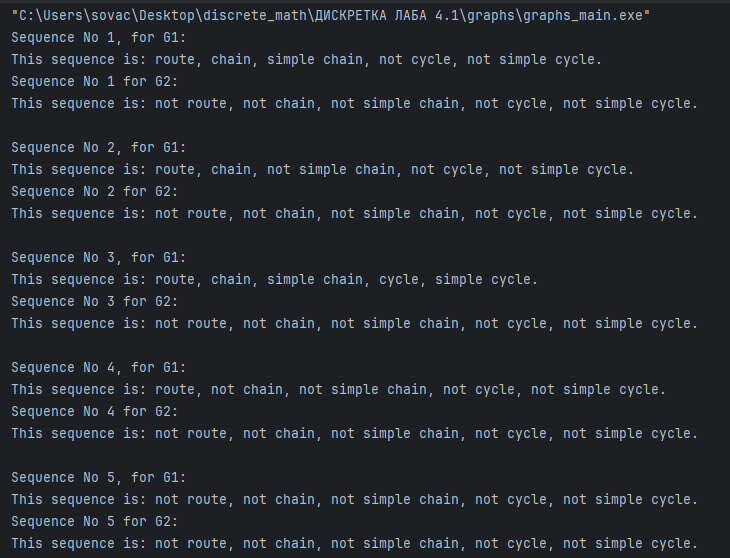
\includegraphics[width=150mm]{images/sequences_properties.png} 
	}
	
	Как мы можем видеть, заключения на экране совпадают с выводами, сделанными в задании 2.
	
	\section{Задание 4}
	\label{task4}

	{\bf Текст задания:} Написать программу, получающую все маршруты заданной длины, выходящие из заданной вершины. Использовать программу для получения всех маршрутов заданной длины в графах $G_1$ и $G_2$ (см. <<Варианты заданий>>, п.а).
	
	Для выполнения этой задачи нам понадобится четыре функции. Первая --- вспомогательная функция вывода последовательности вершин на экран. Вторая --- функция рекурсивного вызова allRoutesWithLenFromVert\_, формирующая маршрут заданной длины и за конкретный вызов задающая значение элемента под индексом cur\_pos в ней (отсчет начинается с нуля). Для этого перебираются все возможные вершины графа, и для каждой проверяется, смежна ли она с последней на текущий момент вершиной в последовательности (то есть включена ли такая пара в матрицу смежности). Если это так, то элемент маршрута под индексом cur\_pos приравнивается к найденному элементу. Затем проверяется, достигла ли последовательность заданной длины: если достигла, то она выводится на экран (с помощью функции printSequence). Иначе рекурсивная функция запускается для тех же данных, но с увеличенным на один индексом cur\_pos. Третья функция, allRoutesWithLenFromVert --- обертка для рекурсивной функции. Она создает последовательность, которая будет формироваться цепочкой рекурсивных вызовов, задает ее первый элемент (он передается функции как аргумент) и запускает рекурсивную функцию с cur\_pos равным 1 (нулевой элемент уже сформирован). Наконец, четвертая функция, allRoutesWithLen, перебирает все возможные вершины графа и вызывая allRoutesWithLenFromVert для каждой из них. Таким образом, на экран выводятся все маршруты заданной длины, а не только начинающиеся с определенной вершины.
	
	В качестве примера вызовем эту функцию сначала для графа $G_1$ и длины 2 (в маршрутах будет 2 ребра и, соответственно, 3 вершины), потом --- для графа $G_2$ и длины 1 (1 ребро, 2 вершины).
	
	\lstinputlisting[linerange={103-135, 214-241, 258-263, 283}]{graphs/graphs_main.c}
	{\centering
	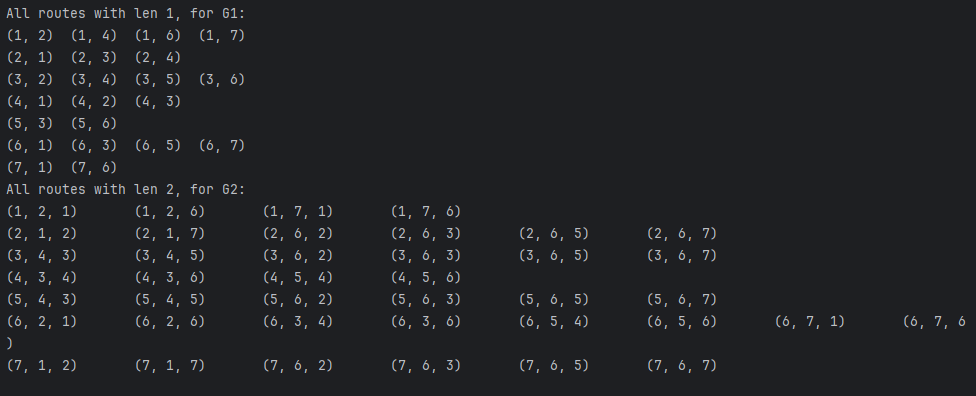
\includegraphics[width=150mm]{images/ex4.png} 
	}
	
	\section{Задание 5}
	\label{task5}
	
	{\bf Текст задания:} Написать программу, определяющую количество маршрутов заданной длины между каждой парой вершин графа. Использовать программу для определения количества маршрутов заданной длины между	каждой парой вершин в графах $G_1$ и $G_2$ (см. <<Варианты заданий>>, п.а).
	
	Воспользуемся упомянутым в лекции свойством, что матрица, в которой элемент на позиции $(i, j)$ указывает, сколько маршрутов заданной длины существует между вершинами $i$ и $j$ для некоторого графа, равна матрице смежности этого графа, возведенной в степень, равную заданной длине. Нам остается лишь реализвать возведение матрицы в степень. В библиотеке для работы с матрицами есть функция умножения матриц, однако в нашем случае использовать ее будет затруднительно, потому что матрица смежности в нашем случае задается не структурой matrix, а массивом целых чисел (отдельное значение задается его конкретным битом). Поэтому возьмем за основу этот алгоритм, но слегка изменим его.
	
	Результирующая матрица будет записываться по переданному функции адресу M. Сначала может показаться, что нам достаточно задать этой матрице начальное значение так, чтобы она была равна исходной матрице смежности, а потом умножать ее на матрицу смежности нужное количество раз. Но если мы будем последовательно перезаписывать каждое значение в результирующей матрице при умножении, то при вычислении значений следующих элементов мы будем опираться на уже перезаписанные, и результаты будут искажены. Поэтому необходимо создать матрицу, хранящую промежуточный результат умножения, и при перезаписи значений результирующей матрицы опираться на нее. 
	
	Таким образом, в функции можно выделить три блока: 1) создание матрицы промежуточного результата и приравнивание ее к исходной матрице смежности, 2) перезапись результирующей матрицы как произведения матрицы смежности и матрицы промежуточного результата, 3) обновление матрицы промежуточного результата и приравнивание ее к результирующей. Шаги 2 и 3 выполняются в цикле до тех пор, пока не будет достигнута степень, равная длине маршрутов, матрицу количества которых мы хотим получить. Для доступа к значениям результирующей матрицы и матрицы промежуточного результата используются ключ values и два индекса, для доступа к значениям матрицы смежности --- функция bin\_relation\_getValue, причем важно учесть, что в обычных матрицах индексы элементов идут с нуля, а в матрице смежности мы используем для обращения значения элементов, идущие с единицы.
	
	В качестве примера вызовем эту функцию дважды для графа $G_2$, сначала для длины 2 (в маршрутах будет 2 ребра и, соответственно, 3 вершины), потом --- для длины 3 (3 ребра, 4 вершины).
	
	\lstinputlisting[linerange={137-161, 214-241, 264-271, 283}]{graphs/graphs_main.c}
	{\centering
	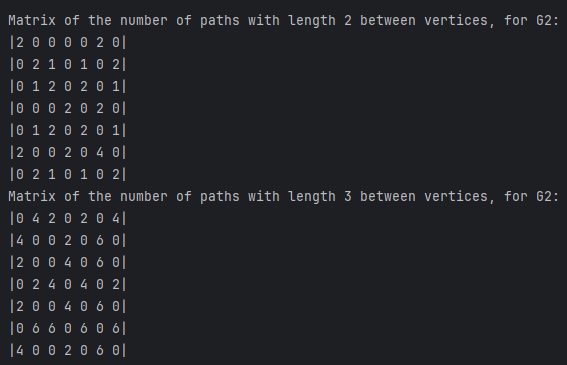
\includegraphics[width=150mm]{images/ex5.png} 
	}
	
	Вручную посчитать все пути из каждой вершины в каждую и проверить, таким образом, истинность этих матриц не представляется возможным, но в принципе результат соответствует здравому смыслу. Например, для длины 2 для каждой вершины количество маршрутов, начинающихся и заканчивающихся в ней самой, равно количеству вершин, с которыми она смежна: формируя маршруты, мы можем перейти в любую из этих вершин и вернуться обратно, и длина маршрута будет составлять ровно 2. Между смежными вершинами же (для этого конкретного графа) нельзя проложить ни одного маршрута длины 2: одно ребро уйдет, чтобы достигнуть этой вершины, второе --- заканчивает маршрут где угодно, но не в этой вершине, а <<обходных>> путей длины 2 к смежным вершинам нет. И наоборот, для длины 3 ни для одной вершины не существует маршрута, начинающегося и заканчивающегося ей самой, зато между смежными вершинами можно проложить не один маршрут. Также можно заметить, что полученные матрицы тоже симметрична --- количество путей из одной вершины в другую будет одинаковым, если поменять местами начало и конец.
	
	\section{Задание 6}
	\label{task6}
		
	{\bf Текст задания:} Написать программу, определяющую все маршруты заданной длины между заданной парой вершин графа. Использовать программу для определения всех маршрутов заданной длины между заданной парой вершин в графах $G_1$ и $G_2$ (см. <<Варианты заданий>>, п.а).
	
	По сути, эта задача сводится к задаче 4: поиску всех маршрутов заданной длины, начинающихся с конкретной вершины --- только теперь в список аргументов добавляется еще одна вершина, которой маршрут должен заканчиваться, и после достижения требуемой длины маршрута необходимо проверить еще одно условие: равна ли последняя вершина полученного маршрута той, которая передана функции как аргумент. Если нет, полученный маршрут не выводится на экран.
	
	В качестве примера вызовем эту функцию дважды для графа $G_2$, сначала для длины 2, начальной вершины 3 и конечной вершины 5, потом --- длины 3, начальной вершины 6 и конечной вершины 5.
	
	\lstinputlisting[linerange={162-182, 214-241, 272-277, 283}]{graphs/graphs_main.c}
	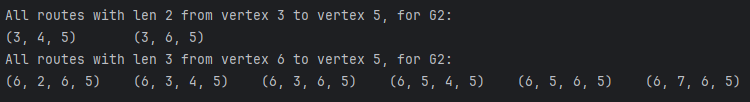
\includegraphics[width=180mm]{images/ex6.png} 
	
	Несложно вручную проследить эти маршруты на графе и убедиться, что они верны. Кстати, можем заметить, что в каждом случае количество выведенных маршрутов совпадает с тем, которое записано в матрицах в задании 5 на соответствующих позициях (строка 3, столбец 5 и строка 6, столбец 5 соответственно).
	
	\section{Задание 7}
	\label{task7}
	
	{\bf Текст задания:} Написать программу, получающую все простые максимальные цепи, выходящие из заданной вершины графа. Использовать программу для получения всех простые максимальных цепей, выходящих из заданной вершины в графах $G_1$ и $G_2$» (см. <<Варианты заданий>>, п.а).
	
	Алгоритм имеет общие черты с таковыми в задачах 4 и 6, однако для него нам потребуется не только хранить простую цепь W, но и сверяться с тем, какие вершины в него уже входили. Можно использовать для этого отдельное множество встреченных вершин V, а можно использовать последовательность, хранящуюся непосредственно в простой цепи W --- ведь если она будет формироваться по правилам, то вершины в ней не будут повторяться; к тому же, если массивы V и W формируются последовательно, то они на каждом шаге, пока условие цепи еще выполняется, будут, по сути, равны. Поэтому логичнее будет оптимизировать программу и использовать только W. 
	
	Для выполнения этой задачи нам понадобится три функции. Первая --- вспомогательная функция, проверяющая, включен ли некоторый элемент в последовательность; она понадобится для проверки сложных условий. Вторая --- функция рекурсивного вызова allMaxSimpleChainsFromVert\_, формирующая максимальную простую цепь и за конкретный вызов задающая значение элемента под индексом cur\_pos в ней (отсчет начинается с нуля). Для этого перебираются все возможные вершины графа, и для каждой проверяется, смежна ли она с последней на текущий момент вершиной в последовательности и не была ли включена в последовательность до сих пор. Если это так, то элемент маршрута под индексом cur\_pos приравнивается к найденному элементу. Затем снова перебираются все возможные вершины, и для каждой, если она смежна с последней, проверяется, входила ли она в последовательность ранее. Если для всех вершин это условие выполняется, то максимальная простая цепь считается сформированной и выводится на экран (с помощью функции printSequence). Иначе рекурсивная функция запускается для тех же данных, но с увеличенным на один индексом cur\_pos. И третья функция, allMaxSimpleChainsFromVert --- обертка для рекурсивной функции. Она создает последовательность, которая будет формироваться цепочкой рекурсивных вызовов, задает ее первый элемент (он передается функции как аргумент) и запускает рекурсивную функцию с cur\_pos равным 1 (нулевой элемент уже сформирован).
	
	В качестве примера вызовем эту функцию сначала для графа $G_1$ и вершины 2, потом --- для графа $G_2$ и вершины 2.
	
	\lstinputlisting[linerange={183-241, 278-283}]{graphs/graphs_main.c}
	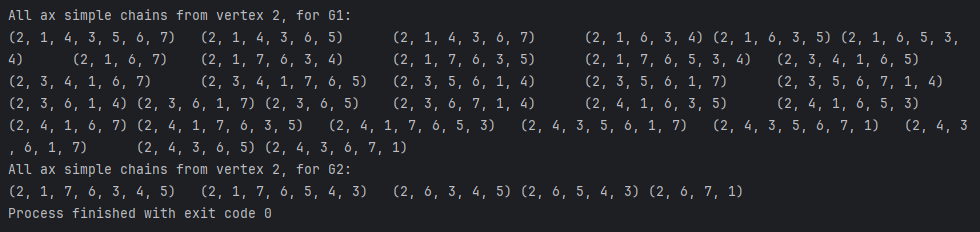
\includegraphics[width=170mm]{images/ex7.png} 
	
	Для графа $G_1$ количество максимальных простых цепей будет слишком велико, чтобы проверить их вручную, но на примере графа $G_2$ мы можем видеть, что они составлены верно. 
	
	Примечание: данный алгоритм не рассматривает замкнутые простые цепи.
	
	\section{Вывод}
	\label{final}
	
	Граф --- пара из множества его вершин и множества связей между ними, то есть двухэлементных подмножеств множества вершин. В ходе данной работы мы анализированы неориентированные графы, не касаясь всего многообразия родственных им объектов: ориентированных графов, мультиграфов, псевдографов, гиперграфов. Граф можно однозначно представить в виде матрицы смежности (элементы матрицы дают информацию о том, смежна ли некоторая пара вершин), матрицы индицентности (элементы матрицы дают информацию о том, инцидентна ли некоторая пара вершины и ребра) и диаграммы (связи между вершинами и ребрами представлены графически). Последовательность попарно перемежающихся вершин и ребер, где соседние элементы инцидентны, задает маршрут в некотором графе. Маршрут можно представить и как последовательность только вершин (или только ребер). Дополнительные свойства маршрутов позволяют выделять среди них цепи, простые цепи, циклы и простые циклы.
	
	В ходе лабораторной работы представили граф тремя разными способами, научились вручную определять, является ли некая последовательность вершин маршрутом, цепью, простой цепью, циклом или простым циклом в конкретном графе, а также написали ряд функций, которые: 1) определяют свойства последовательности вершин относительно конкретного графа, 2) находят все маршруты заданной длины из конкретной вершины, 3) находят все маршруты заданной длины, 4) находят все маршруты заданной длины из конкретной вершины в другую, 5) находят количество маршрутов заданной длины между любой парой вершин, 6) находят максимальные простые цепи из конкретной вершины.

\end{document}